\documentclass[10pt]{article}
\usepackage[a4paper,margin=1.8cm]{geometry}
\usepackage[T1]{fontenc}
\usepackage{lmodern}
\usepackage{microtype}
\usepackage{amsmath}
\usepackage{booktabs}
\usepackage{graphicx}
\usepackage{caption}
\usepackage{float}
\usepackage[hidelinks]{hyperref}
\graphicspath{{figures/}}
\setlength{\parskip}{0.28em}
\setlength{\parindent}{0pt}
\captionsetup{font=small,labelfont=bf,skip=3pt}
\setlength{\textfloatsep}{7pt}
\setlength{\intextsep}{7pt}

\title{\vspace{-1.6em}Sampling cost on a GPU with a smaller cache:\\ BudgetLeafAlias and CodecLeafAlias on an RTX 4050 Laptop}
\author{}
\date{\vspace{-2.4em}}

\begin{document}
\maketitle
\vspace{-1.0em}

\textbf{Summary.} The paper explains the speed of our samplers by where their data is read from, and
notes that it could not check the explanation on a second device: \emph{``All these measurements are
on one GPU; we could not test a GPU with a smaller cache.''} We repeat the paper's two GPU
benchmarks, unchanged and on the same emitter textures, on an RTX 4050 Laptop: the same Ada
multiprocessor, a quarter of them, 24\,MB of L2 instead of 64\,MB, 35\,W instead of 320\,W. (i)~The
L1 limit is the same on both parts, 128--192\,KB, so the 75\,KB structure of $B=4000$ stays inside
it, and on the 1080p emitter BudgetLeafAlias costs a constant $4.2$--$4.3\times$ the paper's figure
at \emph{every} budget --- what a structure that does not change cache level looks like. (ii)~The one
structure that does change level, the 41.5\,MB per-pixel alias table at 1080p, is the one that
degrades: $9.4\times$, more than twice the factor everything else pays, so our margin over it grows
from $1.7\times$ to $3.7\times$. (iii)~$B=4000$ remains the right choice: the paper suggested that
``devices with smaller caches or less memory can use a smaller budget'', and we find that
unnecessary --- in Fireplace a larger budget is actually \emph{cheaper} here. BudgetLeafAlias and
CodecLeafAlias stay the two cheapest samplers in all three scenes, by $1.7$ to $6.5\times$.

\section*{1\quad Setup}

\begin{table}[H]
\centering\small
\begin{tabular}{lll}
\toprule
& RTX 4080 SUPER (paper) & RTX 4050 Laptop (this note) \\
\midrule
Architecture / multiprocessors & Ada (AD103), 80 & Ada (AD107), 20 \\
L1 cache / shared memory per SM & 128\,kB\textsuperscript{a} & 128\,kB \\
L2 cache & 64\,MB\textsuperscript{a} & \textbf{24\,MB}\textsuperscript{c} \\
Device memory / board power & 16\,GB / 320\,W & 6\,GB\textsuperscript{b} / \textbf{35\,W}\textsuperscript{b} \\
SM clock under sustained load & --- & 1665--2340\,MHz\textsuperscript{c} \\
Host CPU & Core i7-14700F\textsuperscript{a} & Core i9-13900H\textsuperscript{b} \\
\bottomrule
\end{tabular}
\caption{\textsuperscript{a}Stated in the paper. \textsuperscript{b}Read from this machine with
\texttt{nvidia-smi}. \textsuperscript{c}Measured here (Section~2 for the L2 capacity). The parts
share the Ada multiprocessor, so L1 is the same size on both; what differs is how many
multiprocessors there are, how much L2 they share, and the power budget.}
\label{tab:gpus}
\end{table}

We do not expect a single scaling factor between these parts: the 4050 has a quarter of the
multiprocessors, about a quarter of the memory interface and a ninth of the power budget. The L2 is
the interesting difference, because the structures the paper measures straddle the two capacities.
The per-texel tables of a 1080p emitter are 16.6\,MB (2D CDF) and 41.5\,MB (per-pixel alias): on the
4080 SUPER both fit inside 64\,MB, while on the 4050 the first fits inside 24\,MB and the second does
not. That is a prediction the paper's explanation makes and this part can test.

\emph{Protocol.} The same \texttt{QuadLightSamplerBench} pass of the same engine. The sampling
benchmark dispatches $1440\times1440$ threads with 128 light samples each; since
$1440^2=2073600=1920\times1080$, this is exactly the paper's ``one $1920\times1080$ frame at 128
light samples per pixel'', with no ray intersection and no shading, and the dispatch alone is timed
with GPU timestamps. The pointer chase walks one random cycle through a buffer growing from 4\,KB to
512\,MB, with $512\times512$ threads of 128 dependent hops. Each configuration runs as a separate
process; we report the median over frames within a process, then over rounds. One deviation was
necessary: this GPU's clock cannot be locked, and at 35\,W it throttles from a 2340\,MHz boost to
about 1665\,MHz, so single runs scatter by up to 40\% in \emph{both} directions, where the paper
reported scatter only on the fast side. Five repetitions of three configurations gave spreads of 1.8\%, 29.0\% and 23.1\%, in
every case from one or two outlying runs while the medians stayed stable and correctly ordered. We
therefore use \textbf{seven rounds instead of the paper's three}; the pointer chase is unaffected,
its round-to-round spread being below 0.5\% everywhere.

\emph{Scenes.} Three of the paper's five scenes can be reproduced here. The emitter textures of
Phone, Fireplace and Convergence survive on this machine and are byte-identical to those the paper
measured, so the comparison is exact rather than approximate; the benchmark reports the emitter as
$1920\times1080$ for Phone and $3840\times2160$ for the other two, as in the paper. Every 4080 SUPER
number below is quoted from the paper and its leaf-budget supplement, not re-measured.

\section*{2\quad The cache hierarchy of this GPU}

\begin{figure}[H]
  \centering
  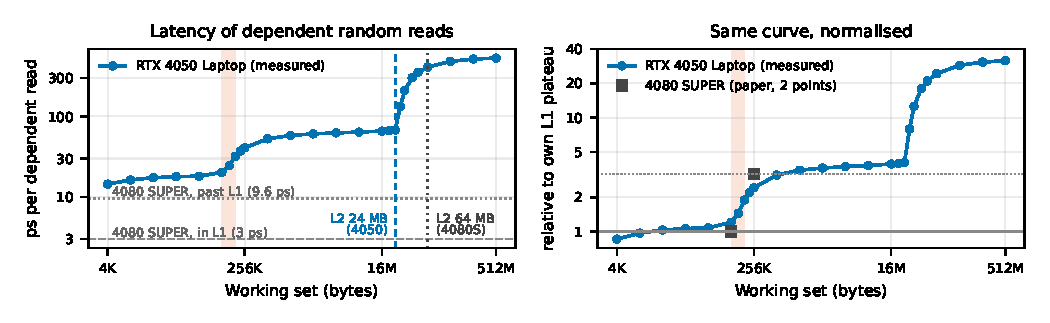
\includegraphics[width=\linewidth]{fig_chase.pdf}
  \caption{Pointer chase. Left: picoseconds per dependent random read, aggregate over the GPU,
  against the size of the data read; horizontal lines are the paper's two values for the 4080 SUPER
  (3\,ps in its L1, 9.6\,ps past it). Shaded: the L1 limit, 128--192\,KB, the same on both parts.
  Right: the same curve over each GPU's own L1 plateau, comparing the \emph{shape} of the hierarchy
  rather than the throughput; grey squares are the paper's $1$ and $3.2\times$.}
  \label{fig:chase}
\end{figure}

The curve has the same three plateaus the paper describes, at different places and heights
(Figure~\ref{fig:chase}). Dependent reads cost 14.4\,ps while the data fits in L1, against 3\,ps on
the 4080 SUPER; that ratio, $4.8\times$, is close to the ratio of multiprocessor counts, which is
what an aggregate throughput should do. The first knee is in the same place on both parts, between
128 and 256\,KB, as it must be since they share the Ada multiprocessor and its 128\,kB of L1: past it
the cost rises to 40.7\,ps, a step of $2.8\times$ against the $3.2\times$ the paper reports. The
second knee is where the parts differ. The L2 plateau holds flat to 24\,MB (67.7\,ps) and then
collapses: 133.5\,ps at 28\,MB, 210.5\,ps at 32\,MB, 409.2\,ps at 64\,MB. \textbf{This is how the
24\,MB in Table~\ref{tab:gpus} is obtained: measured, not quoted from a specification.} Beyond the
cache it settles at 530\,ps, $36.8\times$ the L1 value, matching the paper's ``tens of times more'';
the hierarchy is the same shape with its second step 2.7 times earlier.

\section*{3\quad The cost of a light sample}

\begin{table}[H]
\centering\small
\setlength{\tabcolsep}{4.5pt}
\caption{GPU time of light sampling alone, without ray tracing or shading, for one $1920\times1080$ frame at 128 light samples per pixel, in milliseconds. \emph{4050}: measured on the RTX 4050 Laptop (median of seven rounds). \emph{4080S}: the same measurement on the RTX 4080 SUPER, quoted from Table~2 of the leaf-budget supplement. $\times$: the ratio between the two. The emitter resolution is given per scene.}
\label{tab:cost}
\begin{tabular}{l ccc ccc ccc}
\toprule
 & \multicolumn{3}{c}{Phone (1080p)} & \multicolumn{3}{c}{Fireplace (4K)} & \multicolumn{3}{c}{Convergence (4K)} \\
\cmidrule(lr){2-4}\cmidrule(lr){5-7}\cmidrule(lr){8-10}
Technique & 4050 & 4080S & $\times$ & 4050 & 4080S & $\times$ & 4050 & 4080S & $\times$ \\
\midrule
BudgetLeafAlias $B$=1000 & 48.3 & 11.5 & 4.2 & 101.2 & 11.5 & 8.8 & 67.1 & 11.7 & 5.7 \\
BudgetLeafAlias $B$=2000 & 52.2 & 12.1 & 4.3 & 94.0 & 12.1 & 7.8 & 69.9 & 12.1 & 5.8 \\
BudgetLeafAlias $B$=4000 & 57.6 & 13.3 & 4.3 & 89.1 & 13.2 & 6.7 & 72.7 & 13.1 & 5.5 \\
BudgetLeafAlias $B$=8000 & 60.6 & 14.2 & 4.3 & 86.0 & 14.0 & 6.1 & 77.0 & 14.1 & 5.5 \\
BudgetLeafAlias $B$=16000 & 63.3 & 14.6 & 4.3 & 85.8 & 14.5 & 5.9 & 79.8 & 14.7 & 5.4 \\
CodecLeafAlias & 76.7 & -- & -- & 134.8 & -- & -- & 98.5 & -- & -- \\
2D CDF/8 & 109.7 & -- & -- & 149.6 & -- & -- & 133.6 & -- & -- \\
Mipmap & 179.4 & -- & -- & 196.6 & -- & -- & 181.3 & -- & -- \\
Per-pixel alias & 215.1 & 22.9 & 9.4 & 335.7 & 75.7 & 4.4 & 291.8 & 69.9 & 4.2 \\
2D CDF & 371.7 & 114.8 & 3.2 & 396.0 & 63.8 & 6.2 & 285.8 & 62.1 & 4.6 \\
\bottomrule
\end{tabular}
\end{table}


Read Table~\ref{tab:cost} by its $\times$ columns rather than its milliseconds, since the parts
differ in several ways at once. What the paper's explanation predicts is not that every technique
scales by the same number, but that a technique whose structure \emph{stays in the same level of the
hierarchy} should scale by this part's throughput factor, while one whose structure \emph{falls out
of a level} should scale by more.

\emph{The structure that stays in L1.} On the 1080p emitter of Phone, BudgetLeafAlias costs $4.20$,
$4.32$, $4.33$, $4.27$ and $4.34\times$ the paper's figure at $B=1000$ to $16000$: constant to within
3\% across a structure that grows sixteenfold, from 19\,KB to 300\,KB. This is the signature of a
structure read from the same place on both parts, and the cleanest confirmation of the paper's
argument we can offer --- the 75\,KB of $B=4000$ is in this GPU's L1 exactly as it is on the 4080
SUPER, because that cache is the same size.

\emph{The structure that falls out of L2.} The per-pixel alias table on that emitter is 41.5\,MB. It
fits inside the 64\,MB of the 4080 SUPER and not inside the 24\,MB measured here, and it is the one
entry that degrades out of proportion: $9.39\times$, against the $4.2$--$4.3\times$ BudgetLeafAlias
pays in the same scene --- a penalty of $2.2\times$ on top of everything else. The 2D CDF on that
emitter is 16.6\,MB, still inside 24\,MB, crosses no level and does not pay it ($3.24\times$). On the
two 4K emitters neither per-texel structure crosses a level, since 66\,MB and 166\,MB are outside the
L2 of \emph{both} parts, and accordingly neither shows an extra penalty ($4.2$--$6.2\times$). The
single crossing in the data behaves exactly as the explanation says it should.

\emph{What it costs the baselines.} Our techniques remain the cheapest samplers in every scene. With
$B=4000$ as reference, on this GPU CodecLeafAlias costs $1.33$--$1.51\times$ it, the trimmed 2D CDF
$1.68$--$1.90\times$, the mipmap warp $2.21$--$3.11\times$, the per-pixel alias $3.73$--$4.01\times$
and the dense 2D CDF $3.93$--$6.45\times$. The CodecLeafAlias-to-BudgetLeafAlias ratio,
$1.33$--$1.51$, falls inside the $1.3$--$1.6$ the paper reports, so the relation between our two
techniques is unchanged. Against the per-pixel alias at 1080p our margin grows, from $1.72\times$ to
$3.73\times$; against the dense 2D CDF it narrows, from $8.63\times$ to $6.45\times$, because that
baseline's reads are mostly cache hits on both parts and it loses nothing extra.

\emph{A cost our technique pays at 4K.} BudgetLeafAlias scales by $4.2$--$4.3\times$ on the 1080p
emitter but by $5.4$--$5.8\times$ in Convergence and $5.9$--$8.8\times$ in Fireplace, both 4K. Its
structure is 75\,KB in all three, so the structure is not the cause; what differs is the step every
sampler performs after choosing a texel, reading the emitter's radiance there, from a texture four
times larger. On a part with roughly a quarter of the memory interface that fetch, rather than the
traversal, becomes our sampler's dominant remaining cost --- the honest counterpart to the previous
paragraph: the margin narrows at 4K, for a reason the paper's own framework predicts.

\section*{4\quad The leaf budget}

\begin{figure}[H]
  \centering
  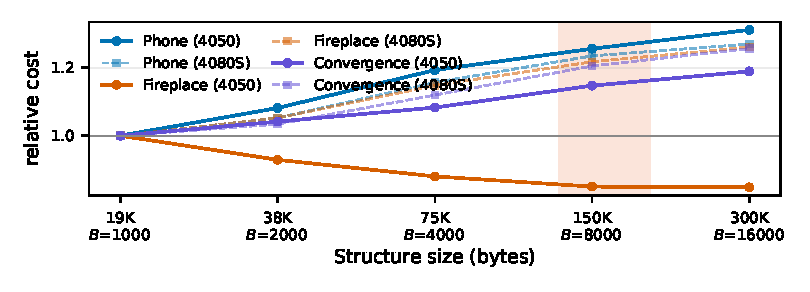
\includegraphics[width=0.46\linewidth]{fig_budget.pdf}
  \caption{Cost against leaf budget, each GPU normalised to its own $B=1000$. Solid: measured here.
  Dashed: the paper's figures. Shaded: the L1 limit, reached by $B=8000$ at 150\,KB.}
  \label{fig:budget}
\end{figure}

The paper chose $B=4000$ at the knee of a quality curve and a cost curve, then hedged: ``devices with
smaller caches or less memory can use a smaller budget at the quality cost shown''. The cost half of
that hedge is unnecessary (Figure~\ref{fig:budget}). From $B=1000$ to $B=16000$ the cost rises by
31\% in Phone against the paper's 27\%, by 19\% in Convergence against 26\% --- and \emph{falls} by
15\% in Fireplace, where the paper measures a 26\% rise.

That inversion is not noise: the spread is 1.3--4.7\% and the medians reproduce to within 0.1\,ms
across seven shuffled rounds (101.2, 94.0, 89.1, 86.0, 85.8\,ms for $B=1000$ to $16000$). The
explanation is the one above. Fireplace has the most concentrated emitter of the three, a small fire
in a 4K frame: a coarse partition gives leaves covering wide areas of that texture, so the radiance
fetches that follow are scattered, while a finer partition clusters the sampled leaves on the fire
and concentrates those fetches into a region that stays in cache. Here the fetch dominates and the
saving outweighs the larger structure; on the 4080 SUPER it is hidden and only the structure shows.
Consistently, Fireplace's scaling factor falls from $8.80\times$ to $5.92\times$ between $B=1000$ and
$16000$, converging on Convergence's.

This reverses the hedge. On this GPU no budget between 1000 and 16000 costs more than 31\% over the
smallest; the quality argument for $B=4000$ is unchanged, being a property of the partition rather
than of the device; and in the one scene where the curves disagree, the smaller budget is the slower
choice. A device with a smaller cache does not need a smaller $B$.

\section*{5\quad Scope}

The explanation survives a change of device, and the claims resting on it hold. Four limitations.
Only three of the five scenes could be run, Rover's and Cinema's emitter videos being absent here;
for the same reason the LED-wall test, where the paper's margin is largest, could not be repeated. We
measure cost only, so nothing here speaks to quality --- which is, however, a property of the
sampling algorithm rather than of the device. The 4080 SUPER column is quoted rather than
re-measured, so it carries that measurement's own conditions, including a lockable clock this part
lacks. Finally, these are isolated dispatches; in a full frame such differences are diluted.

\end{document}
